The model that we discussed about in the previous section gives us a 2D array (x,y) with 17 keypoints per frame. So, the array's form we have at this moment is (N,17,2) where N is the number of frames. However, we want to work in $R^3$ so we have to estimate the third dimension.  Luckily, for us, there is another pre-trained neural network that can solve this problem. This NN takes as input the array that the AlphaPose model estimated (N,17,2) and tries to predict the third dimension, so it returns a new array with form (N,17,3). However, the accuracy of the estimated third dimension drops significantly. \\


Predicting the 3D joint positions of a human body is defined as the task of 3D human pose estimation. The model we chose estimates the relative 3D position of each joint in relation to the root joint. According to the dataset used (COCO) in the previous estimation, the number of joints $N_j$ is set to 17 in this paper.\\

Human3.6M contains 3.6 million video frames for 11 subjects, of which seven are annotated with 3D poses. Each subject performs 15 actions that are recorded using four synchronized cameras at 50 Hz. In our case, which falls under the category of 2D-to-3D estimation there are two methods by which we could convert the 2D keypoints into 3D. Both methods that we are going to discuss, estimate the 3D pose from the 2D pose, using this as the main dataset as a reference.\\

\subsubsection*{Ground-Truth}

Ground truth represents the desired output of an algorithm on an input. The ground truth would be the ideal output you would hope your algorithm can produce. It is also the standard you are defining, by which you evaluate an algorithm. The closer your algorithm is to ground truth the better.\\

In the context of object tracking, the ground truth would represent the 'true' state of the object in each frame. Typically the state of an object is represented by a bounding rectangle which is defined by a width, height, and center, though you can imagine having a simpler or more complicated state depending on the application.\\

For example, in our case we want to track a human in a video sequence. Therefore the ground-truth is going through each frame of the sequence and determining the bounding rectangle that best encloses the human.\\


\begin{figure}[h]
	\centering
	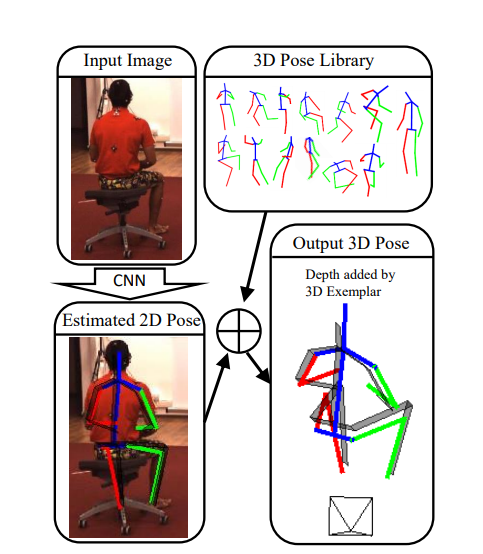
\includegraphics[width=0.75\textwidth]{figures/Implementation/3DModel.png}
	\captionsetup{labelformat=empty}
	\caption{\href{https://arxiv.org/pdf/1811.11742.pdf}
	{The model that takes 2D keypoint sequences (bottom) as input and generates 3D pose
estimates as output (top).}}
\end{figure}


The first method's central idea  \cite{Attention Mechanism Exploits Temporal Contexts: Real-time 3D Human Pose Reconstruction} is to take a sequence of n frames with 2D joint positions as the input and outputs the estimated 3D pose for the target frame as labeled. This model is a fully convolutional architecture with residual connections that takes a sequence of 2D poses as input and transforms them through temporal convolutions.\\

More specifically, this approach does not use heat maps like many other models and instead describes poses with detected keypoint coordinates. This allows the use of efficient 1D convolution over coordinate time series, instead of 2D convolutions over individual heat maps (or 3D convolutions over heat-map sequences). In addition, this idea also makes computational complexity independent of keypoint spatial resolution. This model can reach high accuracy with fewer parameters and allow for faster training and inference. When we loaded the model in our GPU, we used the summary function that is included in the torch library, and it showed that this model has 16,952,371 Trainable parameters. Moreover, we could see the model architecture, in the figure below, again from this function. 


\begin{figure}[h]
	\centering
	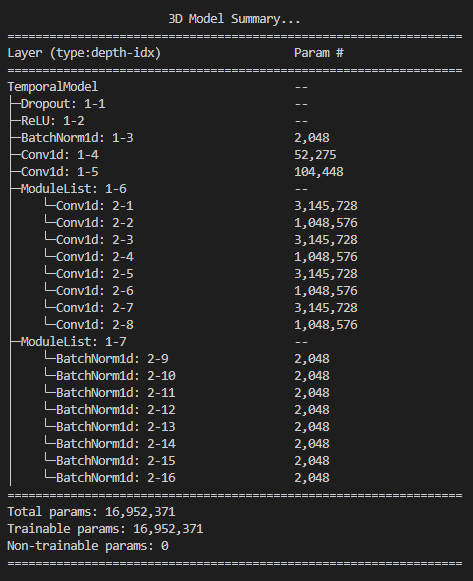
\includegraphics[width=0.6\textwidth]{figures/Implementation/3DModelAr.png}
	\captionsetup{labelformat=empty}
	\caption{3D model summary}
\end{figure}

\pagebreak

\begin{figure}[h]
	\centering
	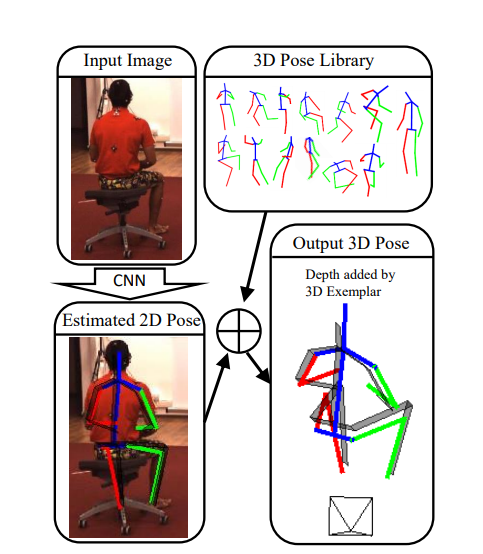
\includegraphics[width=0.65\textwidth]{figures/Implementation/3DModel2Method.png}
	\captionsetup{labelformat=empty}
	\caption{\href{https://arxiv.org/pdf/1612.06524.pdf}
	{3D pose estimation from a 2D estimated pose}}
\end{figure}

The second method's central idea \cite{3D Human Pose Estimation = 2D Pose Estimation + Matching} is to train a neural network to perform 3D pose estimation using both image features from the input image and 2D pose information retrieved from another Neural network (AlphaPose). In other words, this method assumes that the 3D pose X is conditionally independent of the image I, given the 2D pose x, which is not quite true. Given this assumption, we make use of a probabilistic formulation over variables including the image I, the 3D pose $X \in R^{3N}$, and the 2D pose $x \in R^{2N}$ and N is the number of articulated joints. Therefore, we write the joint probability as: 
$$P(X,x,I) = P(X|x) \cdot P(X|I) \cdot P(I)$$
where P(X|I) is a nonlinear function, in our case the AlphaPose model that
predicts the 2D keypoints, and P(X|x) is the Neural network that we will use to estimate the 3D keypoints from the AlphaPose model.\\

Both methods, had great 3D pose reconstruction, while the first method was faster than the second. The first was tested on a single NVIDIA TITAN RTX GPU and for real-time inference, it can reach 3000 FPS, approximately 0.3 milliseconds to process a video frame. In  NVIDIA GeForce GTX 1050 it can reach about 100 FPS, approximately 10 milliseconds to process a video frame. The other method has more complexity since it uses both 2D pose estimation and the image as input. Therefore, the speed was slower, and we decided to choose the faster method since the quality satisfied our needs.\\

So we chose the first model idea, to estimate the 3D human poses from the already estimated 2D. Before this estimation, we normalized all the 2D keypoints. These 2D keypoints were pixels of the image. So we normalized them to have a value between [-1,1] with the below formula:

$$\dfrac{2D_{poses} - \begin{pmatrix} \dfrac{Video_{width}}{2} \ \ ,& \ \dfrac{Video_{height}}{2} \end{pmatrix}}{\begin{pmatrix} \dfrac{Video_{width}}{2} \ \ ,& \ \dfrac{Video_{height}}{2} \end{pmatrix}}$$

Then, after we normalize the 2D poses, we feed them into the model and we get the 3D pose estimation.



